Numerous components go into the process of application development. For a web-application, there is much to consider. What will it look like? What features will it have? What capabilities will the various levels of users have? What kind of database will be used? Where and how will the web-application be hosted? What programming languages will be used? And so on. These questions, and many others, had to be answered thoroughly prior to writing a single line of code. Other things that needed consideration were the needs of the client, the George C. Gordon Library at WPI. Aside from determining which technologies to use for development, it was equally as important to consider the pitfalls of the application we sought to improve and replace.

Our initial meeting with the Gordon Library staff covered what they liked and disliked about LibraryH3lp, the platform they used prior to this project. As they use this platform on a daily basis, a large amount of feedback was provided to us in a short time during the meeting. Most commented on how outdated the elements of the application's interface were and how they felt to use. Additionally, there were numerous features that they felt were missing from the application altogether. Examples of these include the ability to add another staff member to a chatroom with them in the event that the initial staff member who took the chat was not completely comfortable with answering the question presented to them. Another was a major concern where users, or students, were always directed to contact the library directly through live chat, text, phone call, or email when navigating to the 'Contact Us' library web page or 'Lib Guides'. Therefore, in the past, the library staff have received a great number of somewhat simple questions that could have easily been handled without library staff interference whatsoever. They would receive questions on what the library's operating hours were, upcoming events, etc., all topics that are publicly provided on the library's website. To remedy this, the application developed during this MQP would start with replacing the 'Contact Us' page on the library's website to direct users in a manner that could be mostly handled automatically. For instance, if a user had a question of what the library's operating hours were, they would navigate to the library's new 'Contact Us' page, click on 'Library Hours' and be redirected to the page with such information. That way, there is no need to take the time of a library staff member away to answer such a trivial question. The same would be true for other topics such as library hours, news and events, tech suites, alumni, FAQs, and scheduling an appointment with a librarian face-to-face.

Of course, for other concerns such as questions about literature, writing, and other academic affairs would then be welcomed by the 'Email, Call, or Text a Librarian' or 'Live Chat' buttons on the 'Contact Us' page. These adjustments would control the flow in which users interact with the library's website, taking a load off of the library staff's shoulders. Thus, the staff members will have more time to answer more in-depth and pressing questions they may be presented, as well as the other work that they have.

In order to best implement and present these foreseen changes, we chose to use modern programming languages, frameworks, and other technologies to best inhabit our web application. Also, considering all the possible benefits of replacing a subscribed-to platform such as LibraryH3lp, we would develop a nearly free application that would then be hosted on the servers that WPI already have established. That way, the costs for running our application would only lie with data storage and traffic through Amazon Web Services. Though, this would not be much of a concern considering the size of the application and its subsequent data traffic and user base.


%Technologies, things to do the implementation, identifying pitfalls of %current system) (Add lit review here)

Here are some screenshots of LibraryH3lp:

The following is the page all librarians see when they login to LibraryH3lp.
Users are prompted (not shown) for availability to receive messages in each queue (seen in sidebar).
From this page, users can enter chats with other users, or view chats in the queue.

\begin{figure}[H]
    \centering
    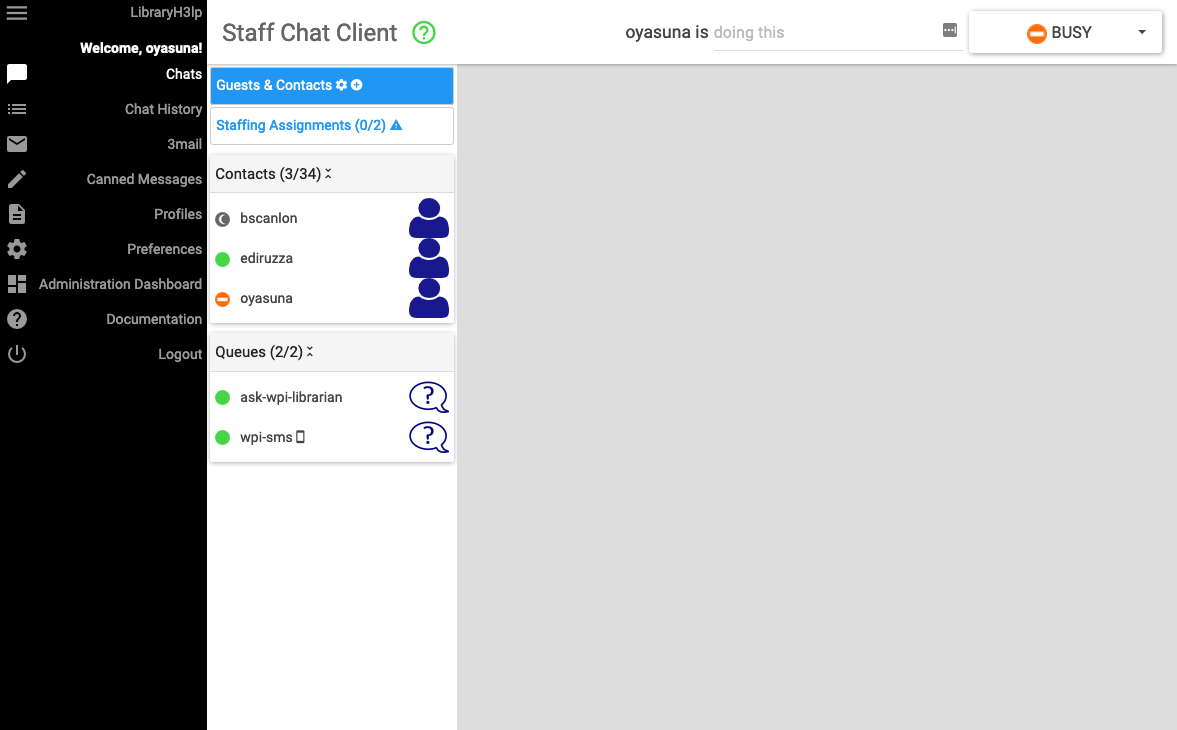
\includegraphics[width=\textwidth]{assets/img/libraryh3lp/libraryh3lp_welcome.png}
    \caption{Librarian welcome view.}
\end{figure}

When a new chat is initiated, users are notified.

\begin{figure}[H]
    \centering
    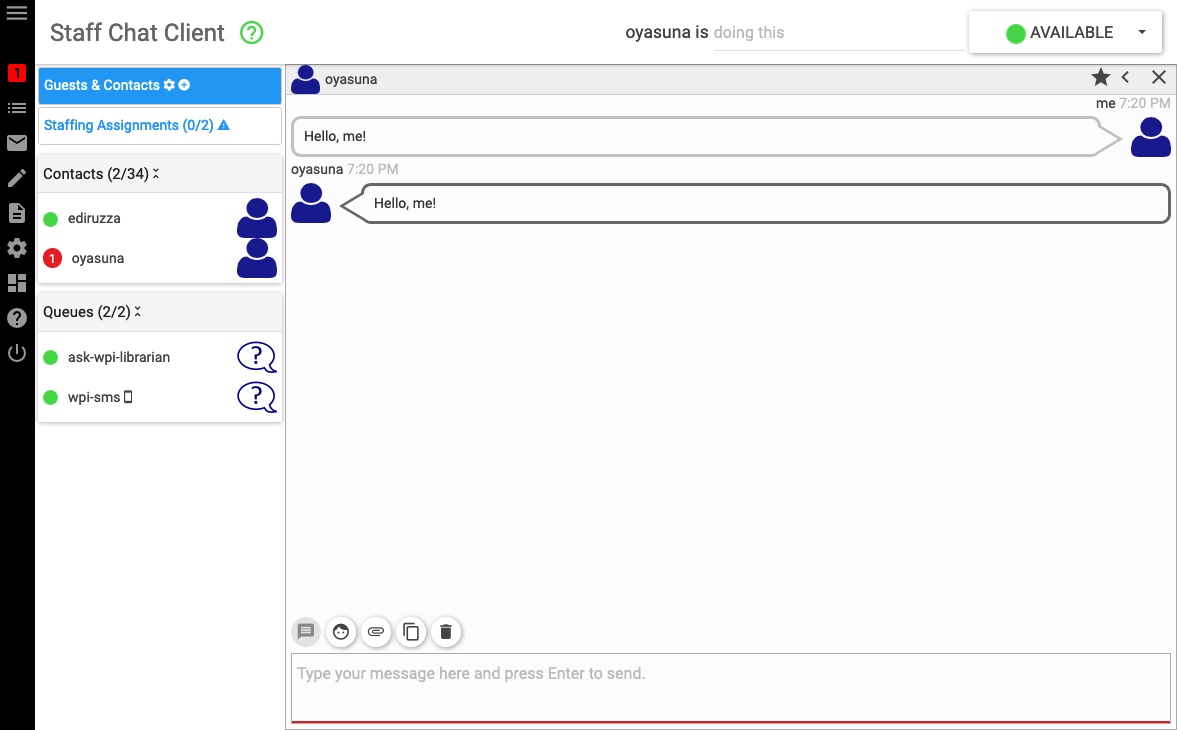
\includegraphics[width=\textwidth]{assets/img/libraryh3lp/me.png}
    \caption{New chat.}
\end{figure}

The following is the view that students see:

\begin{figure}[H]
    \centering
    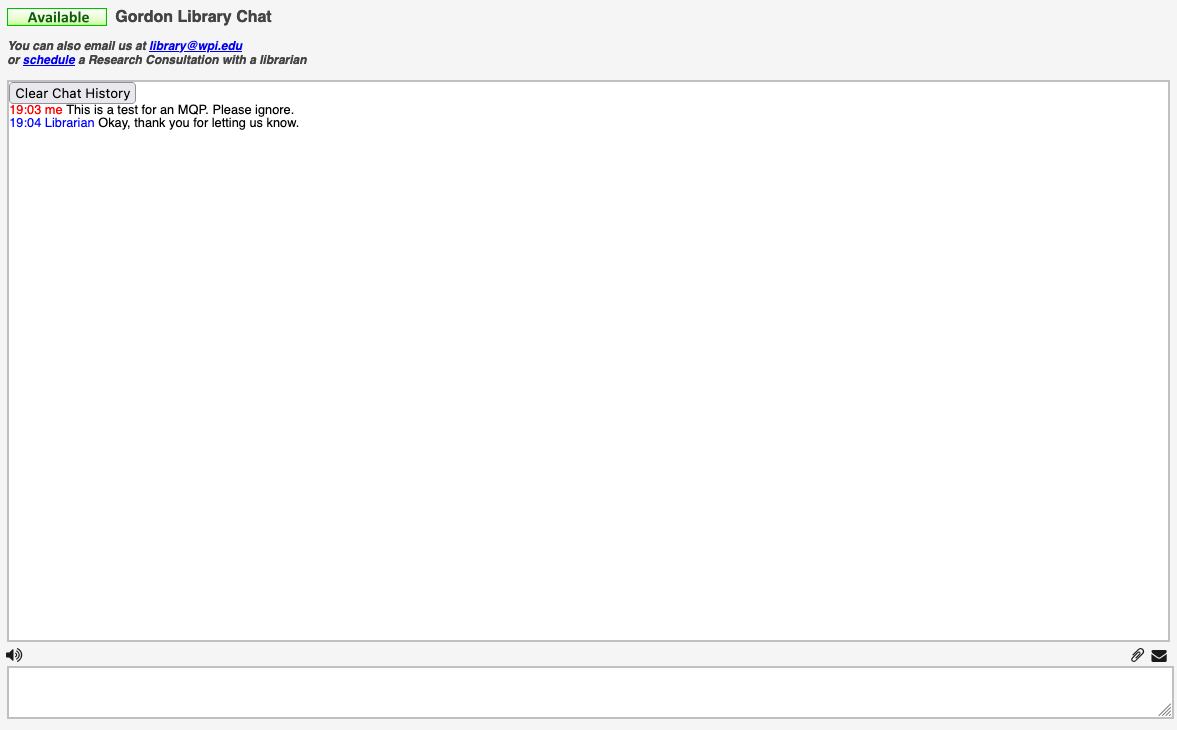
\includegraphics[width=\textwidth]{assets/img/libraryh3lp/libraryh3lp_student_view.png}
    \caption{Student view.}
\end{figure}
